\documentclass[12pt,a4paper]{article}

\usepackage[utf8]{inputenc}
\usepackage[spanish,es-tabla]{babel}
\usepackage[T1]{fontenc}
\usepackage{helvet}
\renewcommand{\familydefault}{\sfdefault}

\usepackage[top=2cm,bottom=2cm,left=2.2cm,right=2.2cm]{geometry}
\usepackage{graphicx}
\usepackage{amsmath,amssymb}
\usepackage{booktabs,tabularx,array}
\usepackage{enumitem}
\usepackage{xcolor}
\usepackage{fancyhdr}
\usepackage{titlesec}
\usepackage{float}
\usepackage{hyperref}

\definecolor{UniBlue}{RGB}{0, 45, 98}
\definecolor{UniRed}{RGB}{140, 29, 34}

\hypersetup{
    colorlinks=true,
    linkcolor=UniBlue,
    citecolor=UniRed,
    urlcolor=UniBlue
}

\newcolumntype{L}{>{\raggedright\arraybackslash}X}

\pagestyle{fancy}
\fancyhf{}
\setlength{\headheight}{15pt}
\fancyhead[L]{\small CC341: Ingeniería de Software (2026--2)}
\fancyhead[R]{\small SIGETUR / PERÚ TOURS}
\fancyfoot[C]{\thepage}
\renewcommand{\headrulewidth}{0.5pt}
\renewcommand{\footrulewidth}{0.4pt}

\titleformat{\section}{\normalfont\large\bfseries\color{UniBlue}}{\thesection}{0.8em}{}
\titleformat{\subsection}{\normalfont\normalsize\bfseries\color{UniBlue}}{\thesubsection}{0.8em}{}
\titleformat{\subsubsection}{\normalfont\normalsize\bfseries\color{black}}{\thesubsubsection}{0.8em}{}
\titlespacing*{\section}{0pt}{1.2ex plus 0.5ex minus .2ex}{0.6ex plus .2ex}
\titlespacing*{\subsection}{0pt}{1.0ex plus 0.4ex minus .2ex}{0.4ex plus .2ex}

\setlist{itemsep=0.15em, topsep=0.2em, parsep=0.1em}

\begin{document}
\pagenumbering{alph}
\begin{titlepage}
    \centering
    \vspace*{0.2cm}
    
    {\Large \textbf{UNIVERSIDAD NACIONAL DE INGENIERÍA}}\\[0.25cm]
    {\large \textbf{FACULTAD DE CIENCIAS}}\\[0.2cm]
    {\normalsize \textbf{ESCUELA PROFESIONAL DE CIENCIA DE LA COMPUTACIÓN}}\\[0.6cm]
    
    
\includegraphics[width=0.20\textwidth]{logo_uni.png}\\[0.6cm]
    
    \rule{\linewidth}{0.5mm}\\[0.35cm]
    {\huge \textbf{PROYECTO SIGETUR}}\\[0.25cm]
    {\Large \textbf{Sistema Integrado de Gestión Turística para PERÚ TOURS}}\\[0.2cm]
    {\normalsize \textbf{Caso de Estudio N° 12}}\\[0.25cm]
    \rule{\linewidth}{0.5mm}\\[0.8cm]
    
    {\large \textbf{CC341 - INGENIERÍA DE SOFTWARE}}\\[0.2cm]
    {\normalsize \textbf{SEMESTRE ACADÉMICO 2026-2}}\\[0.9cm]
    
    \textbf{\Large PRIMERA PRÁCTICA CALIFICADA (PC1)}\\[0.25cm]
    {\large \textit{Artefacto Visión, Modelo del Negocio y Especificación de Requisitos}}\\[1.2cm]
    
    \begin{minipage}{0.88\textwidth}
        \begin{flushleft}
            \textbf{Docente:}\\
            Mg. Zoraida Mamani Rodríguez (\texttt{zmamanir@uni.edu.pe})\\[0.4cm]
            \textbf{Integrantes del Equipo:}\\
            $\bullet$ Berrú Ninahuanca, Sebastián Ángel (\texttt{sebastian.berru.n@uni.pe})\\
            $\bullet$ Huamani Bonifacio, Marco Antonio (\texttt{marco.huamani.b@uni.pe})
        \end{flushleft}
    \end{minipage}
    
    \vfill
    {\normalsize \textbf{Lima, Perú}}\\
    {\normalsize \textbf{Septiembre de 2026}}
\end{titlepage}


\newpage
\pagenumbering{roman}
\tableofcontents
\newpage
\pagenumbering{arabic}

\section{Introducción}
En este informe es para la \textbf{Primera Práctica Calificada (PC1)} de Ingeniería de Software (CC341), correspondiente al ciclo 2026-2 en la Universidad Nacional de Ingeniería, estructuramos bajo la metodología RUP (Rational Unified Process)~\cite{rup2000} % Cita: Libro oficial de RUP (Jacobson, Booch & Rumbaugh)
los tres pilares de la fase de Inicio:

\begin{enumerate}
    \item \textbf{Artefacto Visión:} Problema actual de la agencia, valor frente a los procesos manuales, roles involucrados (stakeholders) y alcance general del sistema.
    \item \textbf{Modelo del Negocio:} Mapeo de cómo opera la agencia según la metodológica de J. García Molina et al.~\cite{garciamolina}, % Cita: Paper metodológico "De los Procesos del Negocio a los Casos de Uso" (Univ. de Murcia)
    definiendo objetivos comerciales, roles externos e internos, procesos clave (CUN) y el flujo de trabajo detallado en carriles (swimlanes).
    \item \textbf{Ingeniería de Requisitos:} Especificación de lo que debe hacer el sistema (Requisitos Funcionales), sus condiciones de calidad y rendimiento bajo FURPS+ (Requisitos No Funcionales) y las políticas operativas de PERÚ TOURS (Reglas de Negocio).
\end{enumerate}

\subsection{Propósito y Alcance del Producto}
El sistema \textbf{SIGETUR} (Sistema Integrado de Gestión Turística)automatiza todo el ciclo de atención comercial de PERÚ TOURS. Su alcance cubre desde registrar a turistas como socios y elaborar cotizaciones personalizadas, hasta negociar los reajustes que solicite el cliente antes del pago. Asimismo, procesa el cobro mediante la pasarela bancaria y genera reportes para gerencia sobre cotizaciones canceladas o aprobadas con cambios en rangos de fechas específicas.

\subsection{Referencias}
\begin{itemize}[noitemsep]
    \item SWEBOK v4: Guide to the Software Engineering Body of Knowledge, IEEE CS, 2024.
    \item García Molina, J. et al.: De los Procesos del Negocio a los Casos de Uso. Univ. de Murcia.
    \item Jacobson, I., Booch, G., \& Rumbaugh, J.: El Proceso Unificado de Desarrollo de Software. Addison-Wesley.
    \item MINCETUR: Reglamento de Agencias de Viajes y Turismo (D.S. N° 005-2020) y Ley N° 29733 de Protección de Datos.
\end{itemize}

\section{Posicionamiento y Planteamiento Estratégico}

\subsection{Planteamiento del Problema (Estándar RUP)}
Actualmente, la agencia \textbf{PERÚ TOURS} gestiona solicitudes y cotizaciones mediante canales desarticulados (hojas de cálculo, correos y mensajería), generando pérdidas de clientes y falta de control gerencial.

\begin{table}[H]
\centering
\footnotesize
\begin{tabularx}{\textwidth}{lX}
\toprule

\textbf{El problema de} & Gestión descentralizada y manual de solicitudes de viaje, lentitud en la presupuestación, falta de trazabilidad en observaciones de cotizaciones y ausencia de métricas sobre cancelaciones. \\ 
\textbf{Afecta a} & Clientes turistas (socios y no socios), Agentes Receptivos y Gerencia de PERÚ TOURS. \\ 
\textbf{Cuyo impacto es} & 
- Demoras de más de 48h en cotizar, perdiendo hasta 30\% de clientes potenciales.\newline
- Observaciones de clientes desatendidas o traspapeladas.\newline
- Desconocimiento gerencial de causas y estacionalidad de cotizaciones canceladas. \\ 
\textbf{Una solución exitosa} & Desarrollar \textbf{SIGETUR}, plataforma web responsive que automatice la afiliación, captura de pedidos de viaje, cotización ágil, diálogo de observaciones, pagos en línea y reportería analítica por fechas. \\ 
\bottomrule
\end{tabularx}
\caption{Declaración formal del problema bajo RUP.}\label{tab:problema}
\end{table}

\subsection{Declaración de Posición del Producto}
\begin{table}[H]
\centering
\footnotesize
\begin{tabularx}{\textwidth}{lX}
\toprule

\textbf{Para} & La agencia de viajes PERÚ TOURS y sus turistas nacionales e internacionales. \\ 
\textbf{Quienes} & Requieren un mecanismo digital rápido y transparente para afiliarse, cotizar a medida y pagar en línea. \\ 
\textbf{El producto SIGETUR} & Es una plataforma web especializada en la gestión del ciclo de vida de cotizaciones turísticas. \\ 
\textbf{Que} & Automatiza desde la afiliación hasta la resolución de observaciones, pagos electrónicos y auditoría. \\ 
\textbf{A diferencia de} & OTAs rígidas (Despegar, Booking) y agencias tradicionales con atención analógica y desordenada. \\ 
\textbf{Nuestro producto} & Permite personalización total de paquetes, negociación directa de observaciones y reportes por fechas. \\ 
\bottomrule
\end{tabularx}
\caption{Declaración de posición del producto.}\label{tab:posicion}
\end{table}

\section{Partes Interesadas y Usuarios}

\subsection{Resumen de Partes Interesadas (No Usuarios Directos)}
\begin{table}[H]
\centering
\footnotesize
\begin{tabularx}{\textwidth}{lLL}
\toprule
\textbf{Parte Interesada} & \textbf{Descripción} & \textbf{Responsabilidades Clave} \\
\midrule
\textbf{Gerente General} & Máxima autoridad ejecutiva y comercial de la agencia. & Validar que el sistema aumente las ventas, reduzca cotizaciones perdidas y cumpla las normas de MINCETUR~\cite{mincetur2020}. \\ % Cita: Reglamento de Agencias de Viajes (D.S. N° 005-2020-MINCETUR)
\textbf{Asesor Legal} & Encargado del cumplimiento normativo de la agencia. & Garantizar que el tratamiento de datos personales y pasaportes cumpla con la Ley N° 29733. \\
\textbf{Administrador TI} & Responsable de servidores, despliegue y soporte técnico. & Mantener el sistema en línea $\ge 99.5\%$, gestionar copias de respaldo y proteger la seguridad de la plataforma. \\
\bottomrule
\end{tabularx}
\caption{Resumen de partes interesadas no usuarias directas.}\label{tab:stakeholders}
\end{table}

\subsection{Resumen de Usuarios Directos del Sistema}
\begin{table}[H]
\centering
\footnotesize
\begin{tabularx}{\textwidth}{lLL}
\toprule
\textbf{Usuario / Rol} & \textbf{Acciones Principales en SIGETUR} & \textbf{Interesado Vinculado} \\
\midrule
\textbf{Cliente No Socio} & Consultar la oferta de viajes y registrarse en la plataforma para convertirse en socio. & Gerente General (captación de nuevos clientes) \\
\textbf{Socio (Turista)} & Solicitar viajes a medida, revisar cotizaciones, enviar observaciones, aprobar presupuestos y pagar en línea. & Gerente General (fidelización y cierre de ventas) \\
\textbf{Agente Receptivo} & Recibir solicitudes de viaje, costear y emitir cotizaciones, aplicar reajustes por observaciones y revisar su historial. & Gerente General (eficiencia y rapidez en la atención) \\
\textbf{Gerente Agencia} & Consultar reportes y métricas de cotizaciones canceladas o aprobadas con cambios en rangos de fechas específicos. & Gerente General (control y toma de decisiones comerciales) \\
\bottomrule
\end{tabularx}
\caption{Resumen de usuarios directos del sistema.}\label{tab:usuarios}
\end{table}

\subsection{Necesidades Clave y Competencia}
\begin{table}[H]
\centering
\scriptsize
\begin{tabularx}{\textwidth}{lcLL}
\toprule
\textbf{Necesidad} & \textbf{Prio.} & \textbf{Situación Actual (Problema)} & \textbf{Solución en SIGETUR} \\
\midrule
Afiliación de Socios & Alta & Registro presencial o correos sin formato que demoran en procesarse. & Registro web con validación automática de datos y cuenta activa al instante. \\
Solicitud de Paquetes & Alta & Mensajes informales por WhatsApp con datos incompletos del viaje. & Formulario estructurado con destino, número de pasajeros y fechas de viaje. \\
Armado de Cotizaciones & Alta & Cálculos manuales en Excel enviados por correo tras días de espera. & Módulo de cotización con cálculo automático de tarifas y márgenes para el agente. \\
Control de Observaciones & Alta & Solicitudes de cambio perdidas o traspapeladas en chats sueltos. & Historial de cambios enlazado a cada cotización para reajustar precios con orden. \\
Cobro en Línea & Alta & Envío de fotos de vouchers bancarios con verificación manual lenta. & Pasarela bancaria integrada con confirmación y liquidación en tiempo real. \\
Auditoría General & Alta & La gerencia no tiene registros de cotizaciones canceladas ni de sus causas. & Reportes filtrados por rango de fechas para auditar cotizaciones canceladas o modificadas. \\
\bottomrule
\end{tabularx}
\caption{Matriz de necesidades clave de los usuarios.}\label{tab:necesidades}
\end{table}

\section{Descripción General del Producto}
SIGETUR se estructura como una plataforma web organizada en tres capas principales:
\begin{itemize}
    \item \textbf{Capa de Presentación (Frontend):} Aplicación web adaptable (\textit{responsive}) accesible desde computadoras de escritorio y dispositivos móviles mediante navegadores modernos.
    \item \textbf{Capa de Negocio y Datos (Backend):} Servicios web RESTful respaldados por una base de datos relacional (PostgreSQL), garantizando la consistencia y seguridad transaccional en cada cotización y pago.
    \item \textbf{Servicios Externos:} Integración con una pasarela de pago bancaria (como Niubiz, Culqi o Stripe) para transacciones en línea y servicios de correo electrónico para el envío automático de cotizaciones y confirmaciones.
\end{itemize}

\subsection{Supuestos y Dependencias}
\begin{enumerate}[noitemsep]
    \item Acceso a conexión a internet estable tanto por parte de los turistas como del personal de la agencia.
    \item Alta disponibilidad ($\ge 99.9\%$) y estabilidad en las APIs de la pasarela de pagos bancaria para procesar los cobros sin interrupciones.
    \item Mantenimiento al día de las tarifas y convenios de PERÚ TOURS con sus proveedores locales (hoteles, transporte y guías turísticos).
\end{enumerate}

\section{Características de Alto Nivel del Producto}
A continuación, se detallan las características principales que delimitan el alcance funcional de SIGETUR y resuelven las necesidades operativas de la agencia:

\begin{table}[H]
\centering
\footnotesize
\begin{tabularx}{\textwidth}{clLcc}
\toprule
\textbf{ID} & \textbf{Característica} & \textbf{Descripción Funcional} & \textbf{Usuario} & \textbf{Prioridad} \\
\midrule
\textbf{C01} & Afiliación de Socios & Registro y validación de nuevos clientes para habilitarlos como socios activos de la agencia. & Cliente No Socio & Alta \\
\textbf{C02} & Solicitud de Paquetes & Ingreso de destino, cantidad de personas, lugares y fechas/horas exactas de partida y regreso. & Socio (Turista) & Alta \\
\textbf{C03} & Emisión de Cotizaciones & Desglose de servicios (transporte, hospedaje, tours) y cálculo de tarifas por el agente. & Agente Receptivo & Alta \\
\textbf{C04} & Aprobación de Cotización & Revisión, comparativa y confirmación de la cotización seleccionada por el cliente. & Socio (Turista) & Alta \\
\textbf{C05} & Gestión de Observaciones & Envío de comentarios, ajustes de presupuesto o cambios de itinerario sobre una cotización recibida. & Socio (Turista) & Alta \\
\textbf{C06} & Procesamiento de Pagos & Cobro electrónico seguro a través de pasarela bancaria para cotizaciones aprobadas. & Socio (Turista) & Alta \\
\textbf{C07} & Auditoría por Fechas & Filtro y generación de reportes sobre cotizaciones canceladas o aprobadas con cambios por rango de fechas. & Gerente / Agente & Alta \\
\bottomrule
\end{tabularx}
\caption{Catálogo de características de alto nivel de SIGETUR.}\label{tab:caracteristicas}
\end{table}

\section{Otros Requisitos del Producto (Modelo FURPS+)}
Los requisitos no funcionales del sistema se clasifican mediante el modelo estándar FURPS+~\cite{pressman2015} % Cita: Clasificación FURPS+ en Ingeniería del Software (Pressman & Maxim)
, asegurando los atributos de calidad y restricciones técnicas que debe cumplir la plataforma: 
\begin{itemize}
    \item \textbf{Usabilidad (Usability):} Interfaz web adaptable (responsive) para computadoras y teléfonos móviles ($\ge 360$\, px) con un flujo simple que permite solicitar un viaje en un máximo de 4 pasos.
    \item \textbf{Confiabilidad (Reliability):} Disponibilidad operativa de al menos $99.5\%$ al mes y copias de seguridad (backups) automáticas diarias de la base de datos para proteger la información comercial.
    \item \textbf{Rendimiento (Performance):} Tiempos de respuesta menores a $1.8$ segundos en la carga de vistas y consultas, con capacidad para atender al menos 100 usuarios concurrentes sin degradar la experiencia.
    \item \textbf{Soportabilidad (Supportability):} Arquitectura modular en capas desacopladas para facilitar mantenimientos futuros y registro de auditoría (logs) protegido contra modificaciones para rastrear cada operación.
    \item \textbf{Seguridad y Restricciones (+):} Conexiones cifradas mediante HTTPS (TLS 1.3), contraseñas almacenadas con algoritmo de hashing robusto (Argon2id) y cobros bancarios procesados por pasarelas con certificación PCI-DSS.
\end{itemize}

\section{Modelo del Negocio}
Antes de especificar el software, se modela el funcionamiento de la agencia PERÚ TOURS siguiendo la metodología de Jesús García Molina et al.~\cite{garciamolina} % Cita: Paper metodológico "De los Procesos del Negocio a los Casos de Uso" (Univ. de Murcia)
. Esto permite alinear los objetivos comerciales, los participantes y los procesos operativos antes de construir el sistema.

\subsection{Objetivos del Negocio (ON)}
Se definen las metas estratégicas que la agencia busca alcanzar con la optimización de sus procesos:
\begin{itemize}[noitemsep]
    \item \textbf{ON-01 (Agilidad):} Reducir el tiempo de armado y entrega de cotizaciones a menos de 4 horas hábiles.
    \item \textbf{ON-02 (Crecimiento):} Aumentar la afiliación de nuevos socios en un 40\% durante el primer año.
    \item \textbf{ON-03 (Conversión):} Recuperar al menos el 25\% de cotizaciones observadas mediante un reajuste ágil de presupuestos.
    \item \textbf{ON-04 (Control):} Lograr el 100\% de registro y trazabilidad de cotizaciones canceladas u observadas para la toma de decisiones gerenciales.
\end{itemize}

\subsection{Actores y Trabajadores del Negocio}
Siguiendo la notación formal de RUP, se diferencian los roles externos de los internos:
\begin{itemize}
    \item \textbf{Actores de Negocio (\texttt{<<Business Actor>>}):} 
    \begin{itemize}[noitemsep] 
        \item \textbf{AN-01 Cliente Turista:} Usuario externo que solicita cotizaciones a medida, negocia cambios y contrata el paquete de viaje.
        \item \textbf{AN-02 Pasarela Bancaria:} Entidad financiera externa encargada de procesar, validar y liquidar los cobros electrónicos.
    \end{itemize}
    \item \textbf{Trabajadores de Negocio (\texttt{<<Business Worker>>}):}
    \begin{itemize}[noitemsep]
        \item \textbf{TN-01 Agente Receptivo:} Operador interno responsable de estructurar las cotizaciones, ajustar costos según observaciones y atender al socio.
        \item \textbf{TN-02 Gerente de Agencia:} Directivo interno responsable de auditar operaciones, revisar cotizaciones canceladas y analizar el desempeño comercial.
    \end{itemize}
\end{itemize}

\subsection{Casos de Uso del Negocio (CUN) y Diagrama}
Representan los procesos fundamentales que aportan valor directo a la organización:

\begin{itemize}[noitemsep]
    \item \textbf{CUN-01: Afiliar Cliente a Socio:} Permite a un turista nuevo registrarse formalmente para acceder a presupuestos y beneficios de socio.
    \item \textbf{CUN-02: Cotizar Paquete Turístico:} Captura los requerimientos del viaje y genera la propuesta económica por parte del agente.
    \item \textbf{CUN-03: Gestionar Venta y Pago de Paquete:} Conduce la negociación de observaciones, la aprobación formal del presupuesto y el cobro en línea.
    \item \textbf{CUN-04: Auditar y Controlar Cotizaciones:} Proceso gerencial para filtrar y evaluar cotizaciones canceladas o modificadas por rango de fechas.
\end{itemize}

\begin{figure}[H]
    \centering
    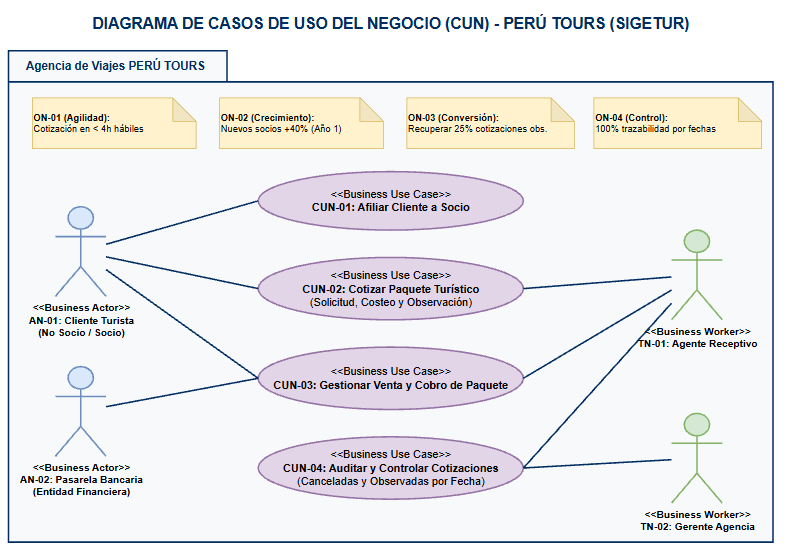
\includegraphics[width=0.85\textwidth]{../diagramas/diagram_cun.png}
    \caption{Diagrama de Casos de Uso del Negocio (CUN) para PERÚ TOURS.}\label{fig:cun}
\end{figure}

\subsection{Diagrama de Actividades con Carriles (Swimlanes)}
El diagrama de actividades detalla la interacción cronológica entre los actores y trabajadores del negocio, separando las responsabilidades por carriles:

\begin{figure}[H]
    \centering
    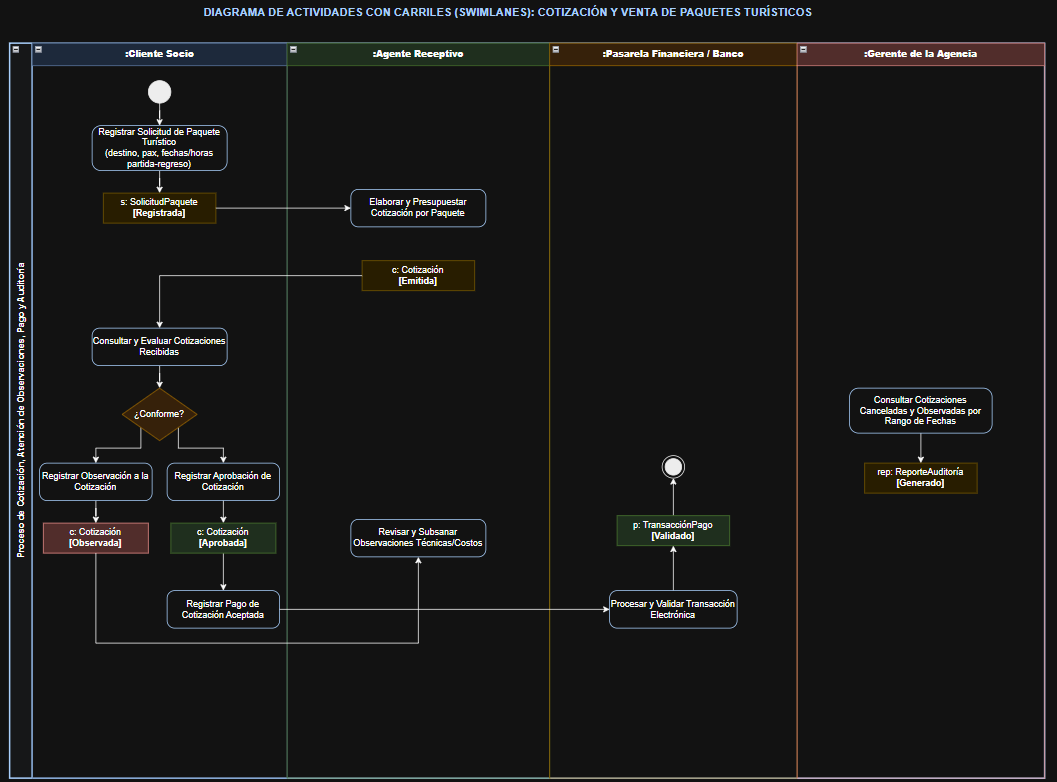
\includegraphics[width=0.88\textwidth]{../diagramas/diagram_actividades.png}
    \caption{Diagrama de Actividades con Carriles y Estados de Objetos del Negocio.}\label{fig:swimlanes}
\end{figure}

\subsubsection{Flujo y Máquina de Estados del Objeto Cotización}
Durante la ejecución de las actividades, el objeto de negocio central \texttt{c: Cotización} transita por los siguientes estados:

\begin{center}
\texttt{[Emitida]} $\longrightarrow$ \texttt{[Observada]} $\rightleftharpoons$ \texttt{[Reajustada]} $\longrightarrow$ \texttt{[Aprobada]} $\longrightarrow$ \texttt{[Pagada]} \quad \text{o bien} \quad $\longrightarrow$ \texttt{[Cancelada]}
\end{center}
\begin{itemize}[noitemsep]
    \item Si el cliente acepta la cotización emitida, pasa de inmediato a \texttt{[Aprobada]} y queda habilitada para el cobro (\texttt{[Pagada]}).
    \item Si el cliente solicita modificaciones, pasa a \texttt{[Observada]}, obligando al agente a generar una versión \texttt{[Reajustada]} hasta lograr la aprobación o llegar a su anulación definitiva (\texttt{[Cancelada]}).
\end{itemize}
\section{Especificación de Requisitos de Software}
Siguiendo las pautas de ingeniería de requisitos del SWEBOK~\cite{swebok2024}, % Cita: Guía del cuerpo de conocimiento de ingeniería de software (IEEE Computer Society)
se formalizan los requisitos del sistema:

\subsection{Requisitos Funcionales (RF)}
\begin{table}[H]
\centering
\footnotesize
\begin{tabularx}{\textwidth}{clLc}
\toprule
\textbf{Código} & \textbf{Requisito Funcional} & \textbf{Descripción Técnica} & \textbf{Rol} \\ \midrule
\textbf{RF01} & Afiliación de Clientes & Registro de clientes no socios mediante formulario web validado. & No Socio \\ \midrule
\textbf{RF02} & Registro de Solicitudes & Captura de destino, n° personas, fechas y horas de partida y regreso. & Socio \\ \midrule
\textbf{RF03} & Emisión de Cotizaciones & Presupuestación de servicios y costos unitarios por el agente receptivo. & Agente \\ \midrule
\textbf{RF04} & Consulta de Cotizaciones & Listado interactivo y comparativa de cotizaciones recibidas. & Socio \\ \midrule
\textbf{RF05} & Aprobación de Cotización & Registro de aceptación formal de cotización seleccionada. & Socio \\ \midrule
\textbf{RF06} & Registro de Observaciones & Ingreso de observaciones descriptivas a cotizaciones de su interés. & Socio \\ \midrule
\textbf{RF07} & Procesamiento de Pago & Cobro digital con pasarela segura y emisión de constancia digital. & Socio \\ \midrule
\textbf{RF08} & Consulta de Auditoría & Filtrado de cotizaciones canceladas o aceptadas con observaciones por rango de fechas. & Gerente / Agente \\ \bottomrule
\end{tabularx}
\caption{Catálogo de Requisitos Funcionales del sistema SIGETUR.}\label{tab:rf}
\end{table}

\subsection{Requisitos No Funcionales (RNF) y Reglas de Negocio (RN)}
\begin{table}[H]
\centering
\footnotesize
\begin{tabularx}{\textwidth}{clL}
\toprule
\textbf{Código} & \textbf{Categoría / Regla} & \textbf{Descripción y Criterio} \\ \midrule
\textbf{RNF01} & Usabilidad & 100\% adaptativo responsive para escritorio y móviles ($\ge 360$ px). \\ \midrule
\textbf{RNF02} & Rendimiento & Tiempos de respuesta $< 1.8$ s en el percentil 95. \\ \midrule
\textbf{RNF03} & Seguridad & Cifrado HTTPS (TLS 1.3), control RBAC y passwords con Argon2id. \\ \midrule
\textbf{RN01} & Condición de Socio & Solo usuarios en estado Socio activo pueden registrar solicitudes y cotizar. \\ \midrule
\textbf{RN02} & Cronología de Viaje & Fecha de regreso estrictamente posterior a fecha de partida ($> 48$h anticipación). \\ \midrule
\textbf{RN03} & Habilitación de Pago & Solo cotizaciones formalmente Aprobadas pueden recibir pagos. \\ \midrule
\textbf{RN04} & Subsanación Observación & Cotizaciones observadas exigen reajuste del agente antes de re-aprobarse. \\ \midrule
\textbf{RN05} & Privacidad de Auditoría & Módulo de auditoría por fechas restringido a Gerente y Agente Receptivo. \\ \bottomrule
\end{tabularx}
\caption{Requisitos No Funcionales y Reglas de Negocio.}\label{tab:rn_rnf}
\end{table}

\subsection{Matriz de Trazabilidad: Negocio vs Requisitos}
\begin{table}[H]
\centering
\footnotesize
\begin{tabularx}{\textwidth}{cLLc}
\toprule
\textbf{Obj. Negocio} & \textbf{Caso Uso Negocio (CUN)} & \textbf{Característica Visión} & \textbf{Requisito (RF)} \\ \midrule
ON-02 & CUN-01 Afiliación de Clientes & C01 Afiliación & RF01 \\ \midrule
ON-01 & CUN-02 Cotizar Paquete & C02 Solicitud Paquete & RF02 \\ \midrule
ON-01 & CUN-02 Cotizar Paquete & C03 Emisión Cotización & RF03 \\ \midrule
ON-01 & CUN-02 Cotizar Paquete & C04 Consulta / Aprobación & RF04, RF05 \\ \midrule
ON-03 & CUN-02 Cotizar Paquete & C05 Registro Observación & RF06 \\ \midrule
ON-01, ON-02 & CUN-03 Venta y Pago & C06 Procesamiento Pago & RF07 \\ \midrule
ON-04 & CUN-04 Auditar Cotizaciones & C07 Auditoría por Fechas & RF08 \\ \bottomrule
\end{tabularx}
\caption{Matriz de trazabilidad integral entre el Negocio y el Software.}\label{tab:trazabilidad}
\end{table}


\newpage
\nocite{*}
\bibliographystyle{plain}
\bibliography{referencias}

\end{document}
